\documentclass[20pt]{beamer}
\mode<presentation>{\usetheme[green]{PosterWUR}}

\usepackage{fontspec}
\setsansfont{DejaVu Sans}
\usepackage[orientation=portrait,size=a0]{beamerposter}
\usepackage{tabularx, booktabs}
\usepackage{hyperref}
\usepackage{qrcode}
%\usepackage{caption}
%\usepackage{subcaption}
\newcolumntype{Y}{>{\centering\arraybackslash}X}

\TPGrid[30mm,30mm]{15}{25}  % 7 - 1 - 7 Columns

\usepackage{graphics}

\title{Change detection in satellite image time series for continuous land cover map updating}
\author{Dainius Masiliūnas¹, Nandin-Erdene Tsendbazar¹, Martin Herold¹, Myroslava Lesiv², Jan Verbesselt¹}


\begin{document}
  \beamertemplatenavigationsymbolsempty
  \begin{frame}{} 

	\begin{textblock}{15}(0,-0.5)
        
\includegraphics[height=0.5\TPVertModule]{figures/Copernicus.jpg} \hskip 1cm
		
\includegraphics[height=0.5\TPVertModule]{figures/PVMEP.png} \hskip 1cm
		
\includegraphics[height=0.5\TPVertModule]{figures/vito-black} \hskip 1cm
		\includegraphics[height=0.5\TPVertModule]{figures/IIASA_PDF}
	\end{textblock}

	\begin{textblock}{7}(0,4)
	  \Line
	  \LHead{1. Introduction}
        \begin{itemize}
         \item Most land cover (LC) maps are produced for a single date
         \item Change processes over time are often more interesting than static land cover
         \item These can be derived from yearly-updated land cover maps, but a class may shift in a different year due to a small shift in model parameters, and not real change on the ground
         \item Dedicated LC change maps are released years after the changes happen, making them suitable for climate but not land management applications
        \end{itemize}
	\end{textblock}
	
	\begin{textblock}{7}(0,7)
	  \Line
	  \LHead{2. Objectives}
        Time series break detection used to:
        \begin{itemize}
         \item Reduce spurious change between year by masking by detected change
         \item Provide the classifier with stable time series (before or after change, not change itself)
         \item Potentially save processing time by not reprocessing unchanged pixels
        \end{itemize}
        
%         Tested break detection methods (in R):
%         \begin{itemize}
%          \item \texttt{strucchange::breakpoints}
%          \item BFAST Monitor
%          \item \textit{t}-test
%         \end{itemize}

	\end{textblock}
	
	\begin{textblock}{7}(0,13.5)
	  \Line 
	  \LHead{3. Input data, methods and validation}
%         Satellite imagery:
%         \begin{itemize}
%          \item MODIS 250 m time series (2009-2019)
%          \item Proba-V 100 m TOC time series (2014-2019)
%          \item Landsat 7+8 30 m time series (2000-2019)
%         \end{itemize}
%         Vegetation indices: NDVI, EVI, NDMI, NIRv.
        MODIS 250m vegetation indices and 3 algorithms used to detect changes, the output of which can then be used to update the map (see Figure \ref{fig-processingchain}). First two algorithms based on Breaks For Additive Season and Trend (BFAST) code at \url{https://github.com/GreatEmerald/bfast}.
        
        Run in two modes (see Figure \ref{fig-updating}):
        \begin{itemize}
         \item Near real-time (NRT) for fast detection of change (BFAST Monitor/\textit{t}-test only)
         \item Consolidated (CONSO) for confirmed change
        \end{itemize}
        
        Validated against a land cover change dataset being collected over Africa (by IIASA and WUR): so far 1010 points over Sahel, additional 607 over Africa, for year 2016. Processing was run on Proba-V MEP Spark cluster at VITO.
    
	  
	\end{textblock}
	
	\begin{textblock}{7}(0,9)
        \begin{figure}
 			\includegraphics[width=7\TPHorizModule]{figures/flowchart-processingchain}
 			\caption{Proposed CGLS-LC100 yearly updated map production chain. Our tested algorithms are combined into a stratification map for reference data collection, and also used in expert rules to filter out spurious change in the classifier/regressor output.}
 			\label{fig-processingchain}
       \end{figure}
	\end{textblock}	
	
	\begin{textblock}{7}(8,3.8)
        \begin{figure}
 			\includegraphics[width=7\TPHorizModule]{figures/flowchart-updating}
 			\caption{Proposed CGLS-LC100 updating process. An NRT map to be released a quarter after the end of the year to be mapped, together with the consolidated map of the year before.}
 			\label{fig-updating}
       \end{figure}
	\end{textblock}	
	
	\begin{textblock}{7}(8,9.25)
		\Line
		\LHead{4. Preliminary results}
		
            %Preliminary results from West African drylands show that land cover change is an uncommon phenomenon, as only 3.4\% of the 1010 reference points show change. All of the tested algorithms tended to overestimate the detected change in this region. The annual t-test algorithm was the fastest, but it does not provide any temporal metrics, only whether there was a break in time series over a chosen year. In contrast, strucchange::breakpoints provides the estimated day of year when a break in the time series is detected. BFAST Monitor is in between, in that it gives a rough estimate of when the break occurred within a particular year.
            
            Tested break detection algorithms tend to detect too much change in West African drylands (3.4\% of the points collected there are real change). When several algorithms are used as confluence of evidence for actual change, much more true change is detected (71.2\%, out of which 61\% was burnt areas and 8\% the change in water extent). Different algorithms perform better or worse depending on the area (see Figure \ref{fig-content}).
            
            Break detection by itself does not give an indication of the class after the change, hence a regularly-updated process from NRT to Consolidated maps is proposed (see Figure \ref{fig-updating}).
            
            Since the difference between yearly classification/regression algorithm outputs by themselves also shows an overestimation of changes, it is useful to combine the two methods to reduce spurious change.
            
            %The algorithms perform better or worse depending on the area, so further tuning of the algorithms is needed, pending collection of more change data. BFAST Monitor and \textit{t}-test runs much faster than \texttt{strucchange::breakpoints}.
		
% 		\begin{figure}
% 		  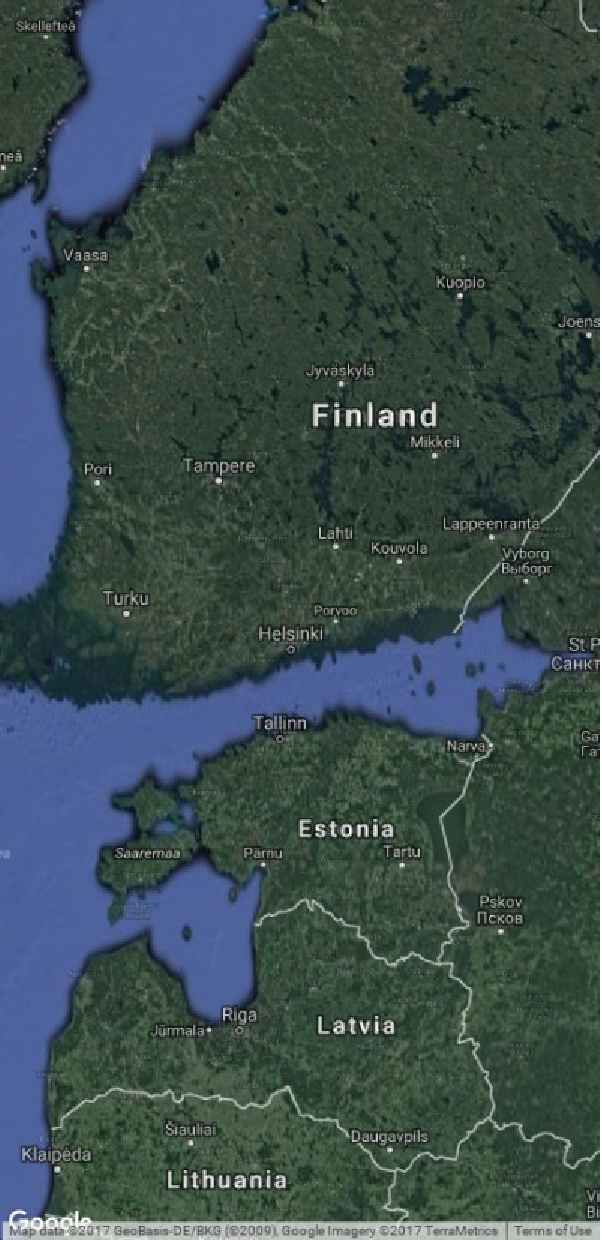
\includegraphics[width=2.3\TPHorizModule]{../thesis/thesis-figures/figures-qgis/fulltile-google}
% 		  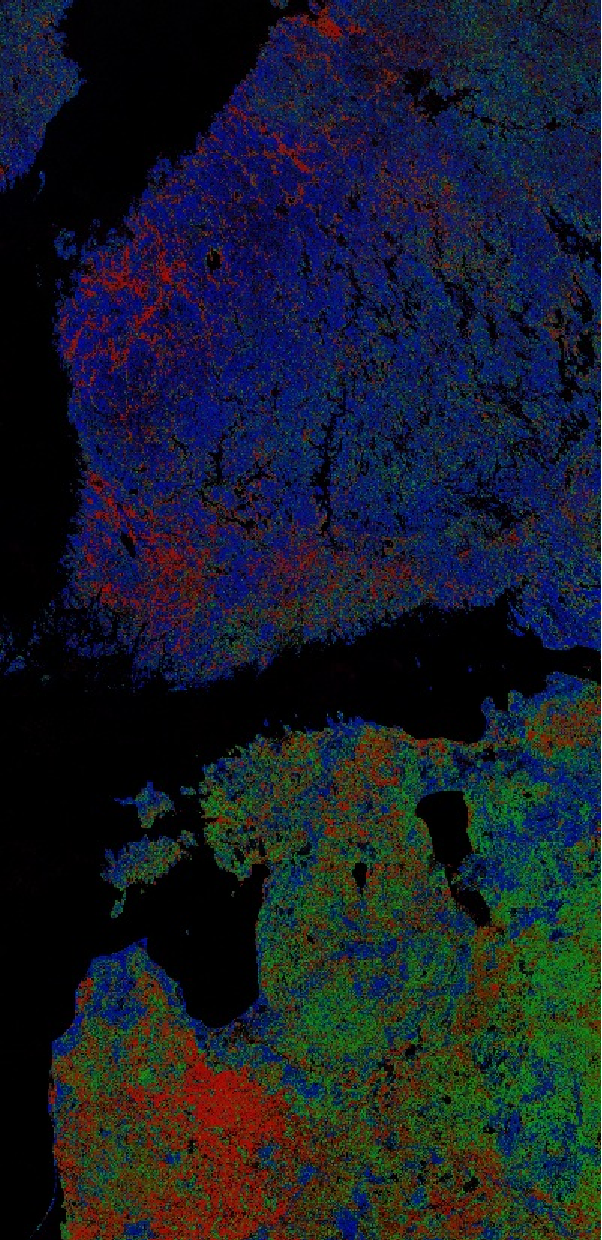
\includegraphics[width=2.3\TPHorizModule]{../thesis/thesis-figures/figures-qgis/fulltile-rf}
% 		  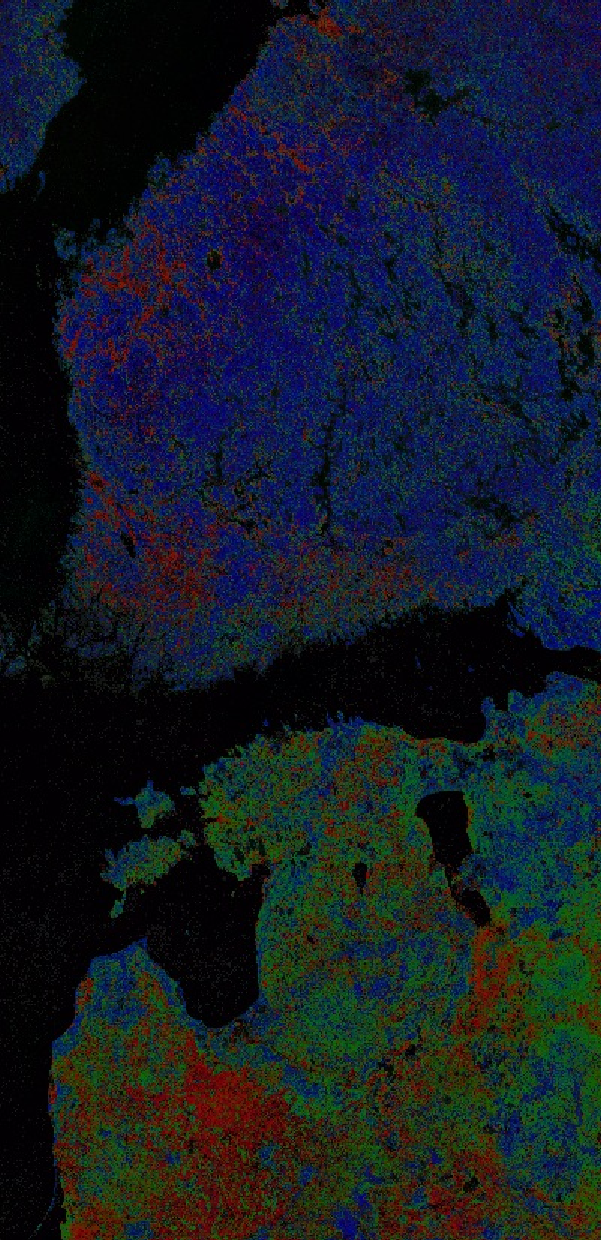
\includegraphics[width=2.3\TPHorizModule]{../thesis/thesis-figures/figures-qgis/fulltile-nn}
% 		  \caption{Results of full-tile fuzzy classification. Left: true colour Google imagery of the study area; middle: random forest regression algorithm; right: neural network algorithm. The colours represent classes: cultivated land (red), deciduous trees (green), evergreen trees (blue).}
% 		\end{figure}
% 		
% 		\begin{figure}
% 		  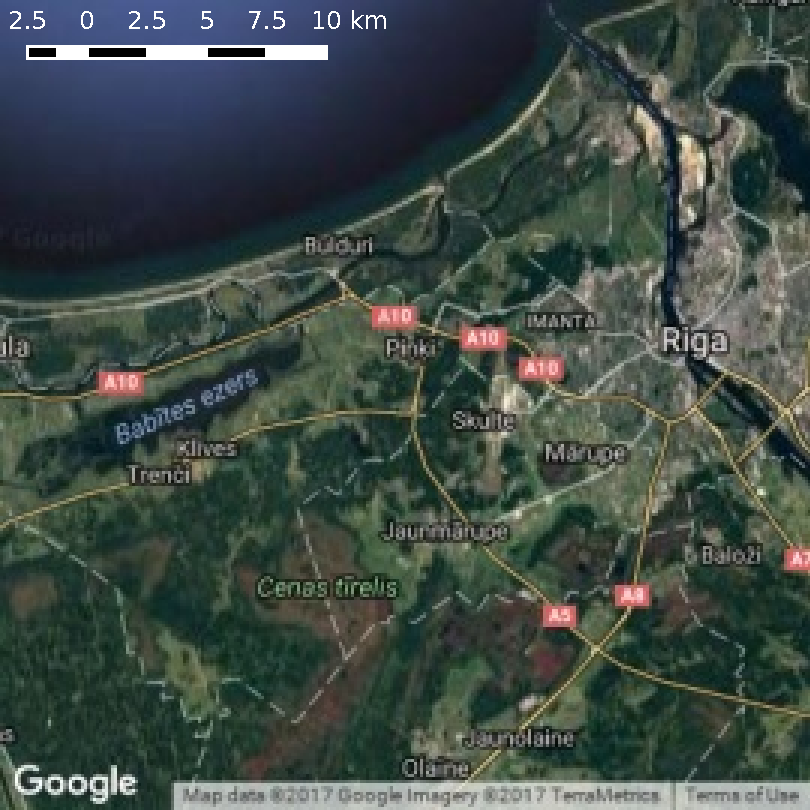
\includegraphics[width=2.3\TPHorizModule]{../thesis/thesis-figures/figures-qgis/riga-google}
% 		  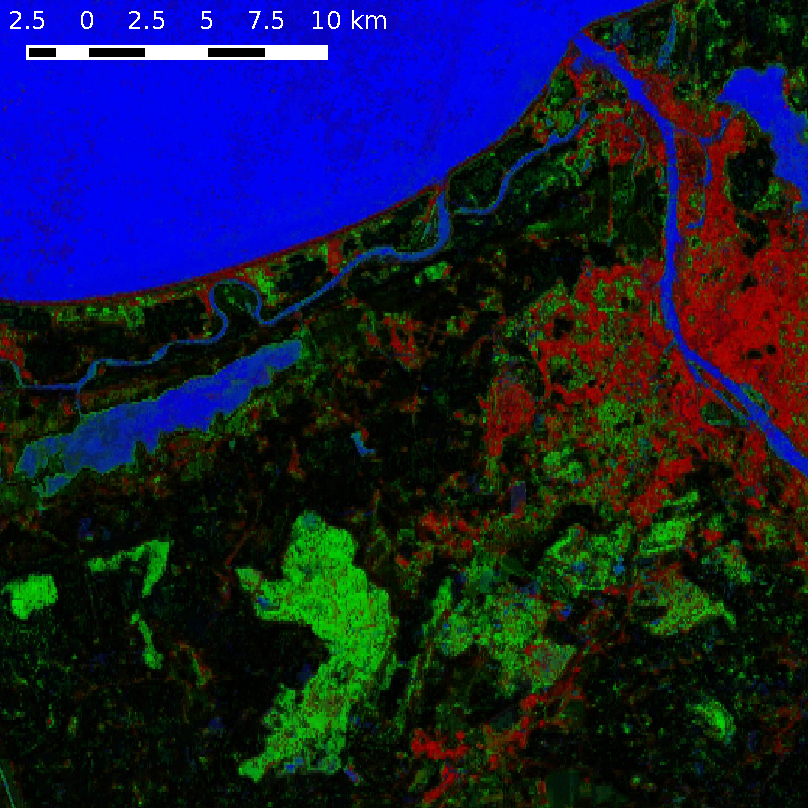
\includegraphics[width=2.3\TPHorizModule]{../thesis/thesis-figures/figures-qgis/riga-rf}
% 		  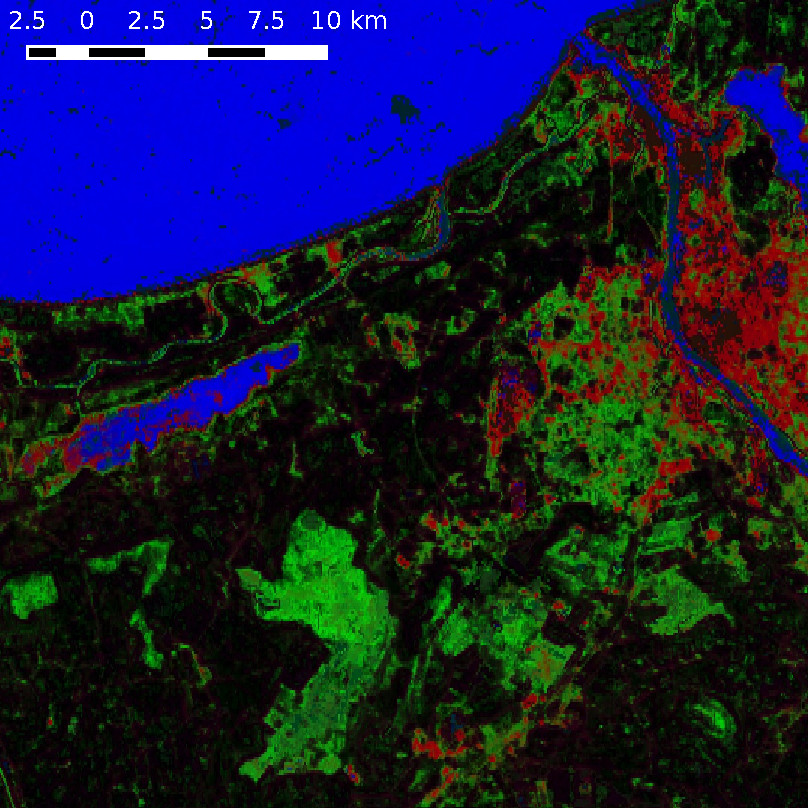
\includegraphics[width=2.3\TPHorizModule]{../thesis/thesis-figures/figures-qgis/riga-nn}
% 		  \caption{Close-up of fuzzy classification in the area surrounding the city of Rīga, Latvia. Left: true colour Google imagery; middle: random forest regression algorithm; right: neural network algorithm. The colours represent classes: built-up (red), wetlands (green), water (blue).}
% 		\end{figure}



	\end{textblock}

	\begin{textblock}{7}(8,13.5)
		\Line
		\LHead{5. Discussion}
            Integrating time-series break detection algorithms help to detect real and immediate land cover changes. Our findings are independent of sensor and thus are applicable for any land cover map updating task, as long as more than 5 years of satellite imagery time series is available. Once finished, it should help improve the production of regularly-updated land cover maps.
            
            One limitation of the updating approach is that the original map is considered accurate (any errors in it will propagate to updated maps). Also, further research on combining the algorithms and vegetation indices is needed to find the optimal map updating strategy, as well as on a methodology to capture changes in land cover fractions, especially gradual (non-break) change.
	\end{textblock}
	
	\begin{textblock}{6}(6.75,23.25)
		%\Line
		\small{\textbf{Acknowledgements}
		
		The research is conducted in close cooperation with the Copernicus Global Land Operations (CGLOPS) project. We would like to thank Marcel Buchhorn, Bruno Smets and Ruben van de Kerchove (VITO) for technical ideas and suggestions, and Proba-V MEP (VITO) for data and computational resources.
		
		Images: Google imagery, Mimi Abebayehu, African Wildlife Foundation.}
		
	\end{textblock}
	
	%\begin{textblock}{7}(8,21)
	%	\Line
	%	\LHead{Acknowledgements}
	%\end{textblock}

	\begin{textblock}{15}(0,17)
        \begin{figure}
 			\includegraphics[width=15\TPHorizModule]{figures/lps19-poster-d11}
 			\caption{Two examples of confirmed land cover change that happened in 2016, and how the changes are detected with the tested algorithms.}
 			\label{fig-content}
       \end{figure}
	\end{textblock}	
	
	\begin{textblock}{15}(0,23)
		\Line
	\end{textblock}	
	
	\begin{textblock}{1}(0,23.5)
		%\begin{figure}
		%\resizebox{1\TPHorizModule}{!}{
		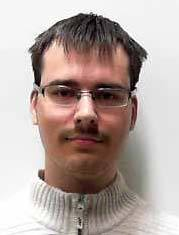
\includegraphics[height=1\TPHorizModule]{figures/dainius.jpeg}
		%} 
		%\end{figure} 
	\end{textblock}
	
	\begin{textblock}{7}(1,23.5)
		%\Adress{
		\small{\color{wursignblue}
            Dainius Masiliūnas\\
			Email: \url{dainius.masiliunas@wur.nl}\\
			LinkedIn: \url{https://www.linkedin.com/in/greatemerald} \\
			ResearchGate: \url{https://www.researchgate.net/profile/Dainius_Masiliunas} \\
			Laboratory of Geo-information Science and Remote Sensing, \url{http://wur.eu/grs}\\
			P.O. Box 47, 6700 AA Wageningen
		}
	\end{textblock}
	
% 	\begin{textblock}{5}(8,23.5)
%         Read full text online: \\ \url{https://edepot.wur.nl/424175} \\
%         Source code: \\ \url{https://github.com/GreatEmerald/master-classification}
% 	\end{textblock}
% 	

    \begin{textblock}{5}(6.75,24.75)
        {\footnotesize ¹: Laboratory of Geo-Information Science and Remote Sensing, Wageningen University \& Research, Wageningen, Netherlands
        
        ²: International Institute for Applied Systems Analysis (IIASA), Laxenburg, Austria}
    \end{textblock}

 	\begin{textblock}{5}(13,23.5)
         \qrcode[height=5cm]{https://www.researchgate.net/profile/Dainius_Masiliunas} \hskip 1cm \qrcode[height=5cm]{https://github.com/GreatEmerald/bfast}
 	\end{textblock}


  \end{frame}
\end{document}
